\documentclass[18pt]{article}
\usepackage{amsmath,amsfonts,amssymb}
\usepackage{natbib}
\usepackage{booktabs}
\usepackage{stmaryrd}
\usepackage{bbold}
\usepackage{nopageno}
\usepackage{bookmark}
\usepackage{pdfpages}
\usepackage[bb=boondox]{mathalfa}
\pagestyle{plain}

\begin{document}
\begin{flushleft}

1 A kernel over subsets
\[
k(A,B)=\begin{cases}
    0 & \text{if } A\cup B =\emptyset \\
    \dfrac{|A \cap B|}{|A\cup B|} & \text{otherwise}
\end{cases}
\]

1. \[ k(A,B)=\begin{cases}
    0 & \text{if } A\cup B =\emptyset \\
    \dfrac{|A \cap B|}{|A\cup B|} & \text{otherwise}
\end{cases}
=\begin{cases}
    0 & \text{if } B\cup A =\emptyset \\
    \dfrac{|B \cap A|}{|B\cup A|} & \text{otherwise}
\end{cases}
=k(B,A)
\]
Hence K is symmetric.\\
\vspace{.4cm}
2. $A_1=\emptyset$, $A_2=\{x_1\}$, $A_3=\{x_2\}$,$A_4=\{x_1,x_2\}$\\
\vspace{.4cm}

\[ K=
\begin{pmatrix}
    0 & 0 & 0 & 0\\
    0 & 1 & 0 & \frac{1}{2}\\
    0 & 0 & 1 & \frac{1}{2}\\
    0 & \frac{1}{2} & \frac{1}{2} & 1
 \end{pmatrix}
\]\\
\vspace{.4cm}
3. Yes, for $n=2$ k can be expressed as $k(A_i,A_j)=\langle \phi(A_i),\phi(A_j)\rangle$.\\
\vspace{.4cm}
By the M.A. theorem this kernel is p.d. and has a corresponding RKHS. The correct mappinps,
$\phi(A_i)$ are printed in the jupyter code below:\\
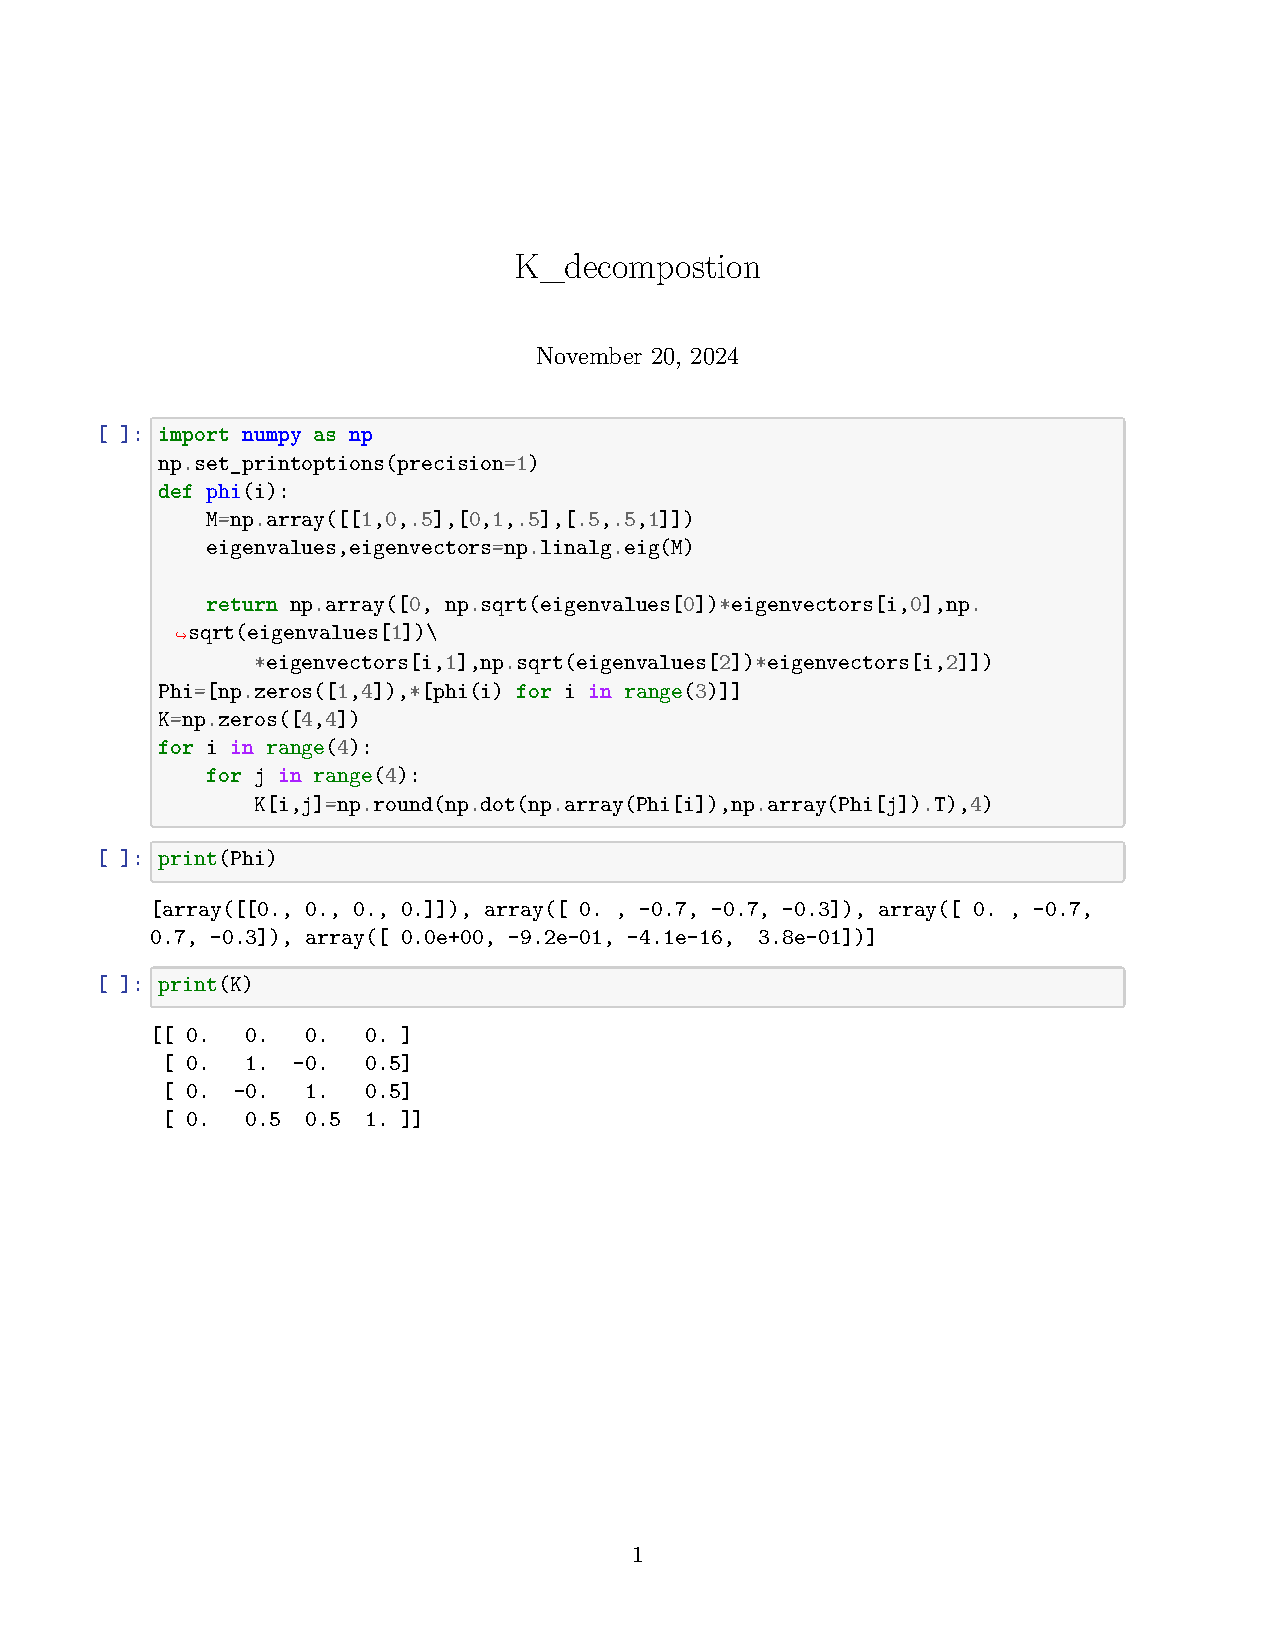
\includepdf{K_decomposition}
\end{flushleft}
\end{document}
